\section{Detailed Methodology}
\label{app:detailed_methodology}

This appendix provides implementation details for Conformal Policy Control. Section~\ref{app:conformal_calibration} describes the calibration procedure for selecting the likelihood ratio bound $\beta$ via weighted conformal prediction, including grid construction, normalization constant estimation, and conformal weighting. Section~\ref{app:sampling} describes sampling algorithms for drawing actions from the constrained policy, including rejection sampling and Independence Metropolis-Hastings.

\subsection{Conformal Calibration of $\beta$}
\label{app:conformal_calibration}


This section details the procedure for calibrating the likelihood ratio bound $\beta$ via weighted conformal risk control. We first define the likelihood ratio and describe how to construct a grid of candidate values (Section~\ref{app:lr_grid_prep}). We then show how to estimate the normalization constant $\psi(\beta)$ for each candidate via importance-weighted Monte Carlo integration (Section~\ref{app:estimating_norm_const}). Finally, we describe the conformal weighting scheme that accounts for distribution shift between calibration and deployment, and the criterion for selecting the largest $\beta$ that controls risk at level $\alpha$ (Section~\ref{app:conformal_weighting}).

\begin{remark}
Throughout this section we write $\pi_0$ for the reference policy used in the likelihood ratio, which generalizes $\pi_0$ from the main text: $\pi_0$ may be the initial safe policy $\pi_0$ or the previous constrained policy $\pi_{t-1}^{(\beta_{t-1})}$. We also assume a fixed context distribution $p(X)$ shared by the safe and optimized policies. Under this assumption, the context marginal cancels in the likelihood ratio $\pi_t(A_i \mid X_i) / \pi_0(A_i \mid X_i)$, and it suffices to work with conditional densities evaluated at the same context $X_i$.
\end{remark}

\subsubsection{Likelihood Ratios and Grid Preparation}
\label{app:lr_grid_prep}

For each action $x$, define the likelihood ratio
\begin{align}
    \mathrm{LR}(x) \coloneqq \frac{\pi_t(x)}{\pi_0(x)},
\end{align}
where $\pi_t$ is the current unconstrained policy and $\pi_0$ is either the initial policy $\pi_0$ or the previous constrained policy $\pi_{t-1}^{(\beta_{t-1})}$.

To calibrate $\beta$, we require two sets of samples:
\begin{itemize}
    \item \textbf{Calibration data} $\mathcal{D}_{\mathrm{cal}}$: samples from previous rounds with feasibility labels, used to compute conformal weights.
    \item \textbf{Proposal data} $\mathcal{D}_{\mathrm{prop}}$: fresh samples from $\pi_t$, used to estimate the normalization constant $\psi(\beta)$.
\end{itemize}

We construct a grid $G$ of candidate $\beta$ values from the observed likelihood ratios across both datasets:
\begin{align}
    G = \textsc{PrepareGrid}\left(\{\mathrm{LR}(x) : x \in \mathcal{D}_{\mathrm{cal}} \cup \mathcal{D}_{\mathrm{prop}}\}\right).
\end{align}
The grid is sorted in increasing order, and we search from the most conservative (smallest $\beta$) to the most permissive, stopping at the first $\beta$ where the weighted infeasibility rate exceeds $\alpha$. See Figure~\ref{fig:beta_calibration} for an illustration.

\begin{figure}[!ht]
    \centering
    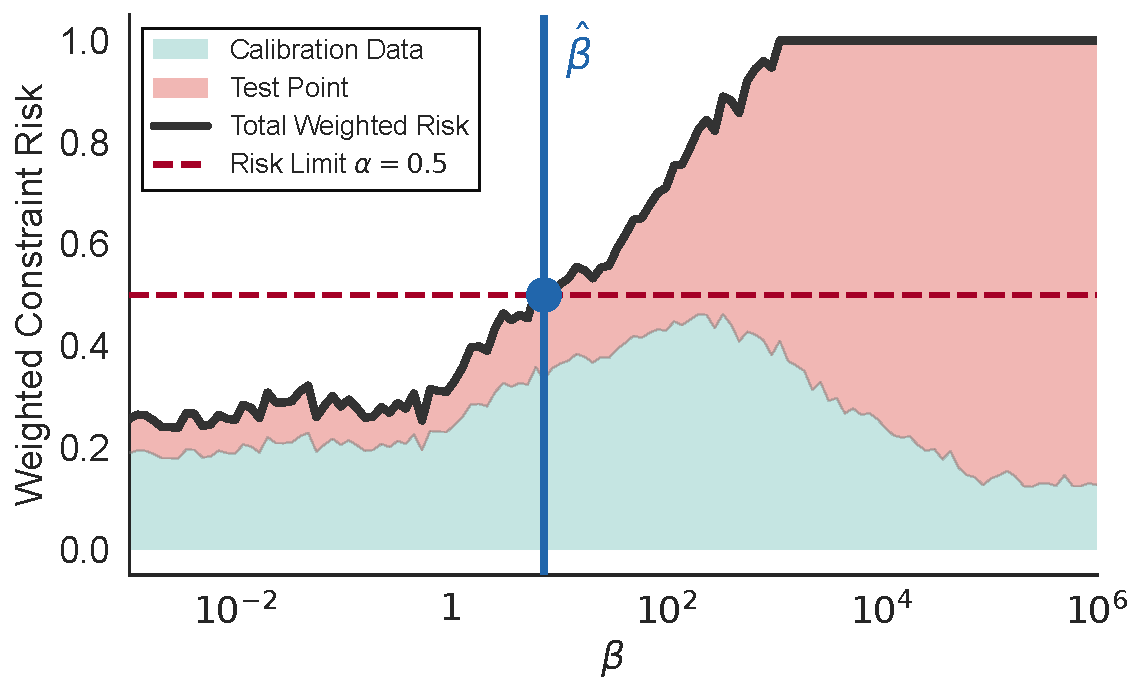
\includegraphics[width=0.5\linewidth]{figures/cpc_conformal_weighting.pdf}
    \caption{An illustration of fitting $\hat \beta$ to calibration data drawn from $\pi_0$. We draw a test point from the optimized policy and conservatively assume the loss attains the upper bound $B$. As $\beta$ increases, the contribution of the test point to the weighted average constraint violation increases. We search $\beta$ in increasing order, recomputing the conformal weights for each setting of $\beta$ and halting at the first point $\hat \beta$ where the average constraint violation exceeds $\alpha$.}
    \label{fig:beta_calibration}
\end{figure}


\subsubsection{Estimating the Normalization Constant $\psi(\beta)$}
\label{app:estimating_norm_const}

Recall that the constrained policy is defined as
\begin{align}
    \pi^{(\beta)}(x) = \frac{\min\{\pi_t(x), \beta \cdot \pi_0(x)\}}{\psi(\beta)},
\end{align}
where $\psi(\beta) = \int \min\{\pi_t(x), \beta \cdot \pi_0(x)\} \, dx$ is the normalization constant. We estimate $\psi(\beta)$ via importance-weighted Monte Carlo integration using the proposal data $\mathcal{D}_{\mathrm{prop}}$.

When sampling from the optimistic policy $\pi_t$:
\begin{align}
    \psi(\beta)
    &= \mathbb{E}_{\pi_t}\left[\frac{\min\{\pi_t(x), \beta \cdot \pi_0(x)\}}{\pi_t(x)}\right]
    = \mathbb{E}_{\pi_t}\left[\min\left\{\frac{\beta}{\mathrm{LR}(x)}, 1\right\}\right] \\
    &\approx \frac{1}{|\mathcal{D}_{\mathrm{prop}}|} \sum_{x \in \mathcal{D}_{\mathrm{prop}}} \min\left\{\frac{\beta}{\mathrm{LR}(x)}, 1\right\}.
\end{align}

When sampling from the safe policy $\pi_0$:
\begin{align}
    \psi(\beta)
    &= \mathbb{E}_{\pi_0}\left[\frac{\min\{\pi_t(x), \beta \cdot \pi_0(x)\}}{\pi_0(x)}\right]
    = \mathbb{E}_{\pi_0}\left[\min\left\{\mathrm{LR}(x), \beta\right\}\right] \\
    &\approx \frac{1}{|\mathcal{D}_{\mathrm{prop}}|} \sum_{x \in \mathcal{D}_{\mathrm{prop}}} \min\left\{\mathrm{LR}(x), \beta\right\}.
\end{align}

In practice, all computations are performed in log space for numerical stability. Writing $r_i = \log \mathrm{LR}(x_i)$ for each sample, the log normalization constant is
\begin{align}
    \log \psi(\beta) = \mathrm{logsumexp}\left(\{\min(\log \beta - r_i, 0)\}_{i=1}^{n}\right) - \log n
\end{align}
for the optimistic proposal, and similarly with $\min(r_i, \log \beta)$ for the safe proposal.

\subsubsection{Conformal Weighting}
\label{app:conformal_weighting}

The calibration data $\mathcal{D}_{\mathrm{cal}}$ is drawn from a mixture of policies across previous rounds. To apply conformal prediction under this distribution shift, we weight each calibration point by the likelihood ratio between the candidate constrained policy and the calibration mixture:
\begin{align}
    \tilde{w}_i(\beta) = \frac{\pi^{(\beta)}(x_i)}{\pi_{\mathrm{mix}}(x_i)}, \quad x_i \in \mathcal{D}_{\mathrm{cal}},
\end{align}
where $\pi_{\mathrm{mix}}$ is the mixture distribution over previous constrained policies, weighted by the number of calibration samples from each round.

For the test point, we use a conservative upper bound by taking the maximum weight over the proposal samples:
\begin{align}
    \tilde{w}_{\mathrm{test}}(\beta) = \max_{x \in \mathcal{D}_{\mathrm{prop}}} \frac{\pi^{(\beta)}(x)}{\pi_{\mathrm{mix}}(x)}.
\end{align}

We normalize all weights to sum to one:
\begin{align}
    w_i(\beta) = \frac{\tilde{w}_i(\beta)}{\sum_{j} \tilde{w}_j(\beta) + \tilde{w}_{\mathrm{test}}(\beta)}, \quad
    w_{\mathrm{test}}(\beta) = \frac{\tilde{w}_{\mathrm{test}}(\beta)}{\sum_{j} \tilde{w}_j(\beta) + \tilde{w}_{\mathrm{test}}(\beta)}.
\end{align}

Let $B$ denote the upper bound on the loss $\ell(x)$. The weighted risk estimate is
\begin{align}
    \hat{R}(\beta) = \sum_{i \in \mathcal{D}_{\mathrm{cal}}} w_i(\beta) \, \ell(x_i) + w_{\mathrm{test}}(\beta)\cdot B,
\end{align}
where the test point is conservatively assigned the worst-case loss $B$. We select $\hat{\beta}$ as the largest value in the grid $G$ such that $\hat{R}(\beta) \leq \alpha$.

\subsection{Sampling from the Constrained/Risk-Controlling Policy}
\label{app:sampling}


In this section, we describe three approaches to sample from $\pi^{(\beta)}$: rejection sampling with either $\pi_0$ or $\pi_t$ as the proposal (Section~\ref{app:rejection_simple}), rejection sampling with a mixture proposal (Section~\ref{app:rejection_mixture}), and Independence Metropolis-Hastings (Section~\ref{app:imh}).

\subsubsection{Rejection Sampling with Simple Proposals}
\label{app:rejection_simple}

We first review the classic accept-reject procedure. Let $\tilde p(x)$ be an unnormalized target density and $q(x)$ a normalized proposal such that
$$\frac{\tilde p(x)}{q(x)} \leq M \quad \forall x,$$
for some envelope constant $M < \infty$.\footnote{Alternatively, we can view $M q(x)$ as the unnormalized envelope proposal with normalizing constant $M$.} To sample from $p(x) = \tilde p(x) / \int \tilde p(x) dx$, we proceed as follows: draw $X \sim q$, draw $U \sim {\rm Unif}(0, 1)$, and accept $X$ if $U \leq \frac{\tilde p(X)}{M q(X)}$. The optimal (smallest) envelope constant is
$$M^\star = \sup_x \ \frac{\tilde p(x)}{q(x)}.$$

The marginal acceptance probability is
\begin{align}
\mathbb{P} \left[U \leq \frac{\tilde p(X)}{M q(X)} \right] 
&= \mathbb{E} \left[ \mathbbm{1} \left\{U \leq \frac{\tilde p(X)}{M q(X)} \right\} \right] \nonumber \\
&= \mathbb{E} \left[ \mathbb{E}\left[ \mathbbm{1} \left\{U \leq \frac{\tilde p(X)}{M q(X)} \right\} \Big| X \right] \right] \nonumber \\
&= \mathbb{E} \left[ \mathbb{P}\left[ U \leq \frac{\tilde p(X)}{M q(X)}  \Big| X \right] \right] \nonumber \\
&= \mathbb{E}_{X\sim q}\left[\frac{\tilde p(X)}{M q(X)} \right] \nonumber \\
&= \int_{x: q(x)>0} q(x) \frac{\tilde p(x)}{M q(x)} dx \nonumber \\
&= \frac{1}{M}\int_{x: q(x)>0} \tilde p(x) dx
\label{eq:app:accept_prob_rejection_sampling}
\end{align}
so tighter $M$ leads to higher acceptance rates.

\paragraph{Safe policy proposal.} Take $\tilde p(x) = \tilde \pi^{(\beta)}(x) = \min\{ \pi_t(x), \beta \pi_{\rm safe}(x) \}$ and $q(x) = \pi_{\rm safe}(x)$. Then for all $x$,
$$
\frac{\tilde p(x)}{q(x)} = \min \left\{ \frac{\pi_t(x)}{\pi_{\rm safe}(x)}, \beta \right\} \leq \beta,
$$
so we choose $M = \beta$. The pointwise acceptance probability then is
\begin{equation}
\frac{\tilde p(x)}{\beta \pi_{\rm safe}(x)} = \min\left\{\frac{\pi_t(x)}{\beta\pi_{\rm safe}(x)}, 1 \right\},
\label{eq:app:accept_prob_safe_proposal}
\end{equation}
or $\frac{\pi_t(x)}{\beta\pi_{\rm safe}(x)}$ in the unclipped region and $1$ in the clipped region.

\paragraph{Optimized policy proposal.} If we instead take $q(x) = \pi_t(x)$, then for all $x$,
$$
\frac{\tilde p(x)}{q(x)}
=
\frac{\min\{\pi_t(x),\,\beta\pi_{\rm safe}(x)\}}{\pi_t(x)}
=
\min \left\{1, \frac{\beta\pi_{\rm safe}(x)}{\pi_t(x)} \right\}
 \leq 1,
$$
so we may take $M=1$.
The pointwise acceptance probability is
\begin{align}
\frac{\tilde p(x)}{\pi_t(x)}
=
\min\left\{1, \frac{\beta\pi_{\rm safe}(x)}{\pi_t(x)} \right\},
\label{eq:app:accept_prob_opt_proposal}
\end{align}
which is $1$ in the unclipped region and $\frac{\beta\pi_{\rm safe}(x)}{\pi_t(x)}$ in the clipped region.


Intuitively, the relative efficiency of the two proposals depends on the constraint parameter $\beta$ controlling how much the optimized policy is truncated toward the safe policy. When $\beta$ is small, the constrained target resembles a rescaled version of $\pi_{\rm safe}$ over most of its support. Proposing from $\pi_{\rm safe}$ tends to be efficient in this regime, because most points satisfy $\pi_t(x)/\pi_{\rm safe}(x) \ll \beta$ and the acceptance probability in \autoref{eq:app:accept_prob_safe_proposal}, while small, varies smoothly over $x$. In contrast, proposing from $\pi_t$ can be inefficient with small $\beta$, since $\pi_t$ may place substantial mass in regions that are heavily downweighted by the constraint, leading to frequent rejections.


When $\beta$ is large, the constrained target resembles $\pi_t$. As long as $\pi_t(x) / \pi_{\rm safe}(x) \lesssim \beta$ for most of the support of $\pi_t$, then using $\pi_t$ as the proposal tends to be more efficient in this regime, as the acceptance probability in \autoref{eq:app:accept_prob_opt_proposal} is frequently close to $1$. If, however, $\pi_t$ concentrates mass in regions where $\pi_t(x) / \pi_{\rm safe}(x)$ is extremely large, this proposal can still perform poorly.


At intermediate values of $\beta$, neither proposal dominates. The constrained target may allocate comparable mass from $\pi_{\rm safe}$ and $\pi_t$. Both proposals can suffer from mismatches with different parts of the target, motivating the use of mixture proposals that adaptively trade off between $\pi_{\rm safe}$ and $\pi_t$.

\subsubsection{Rejection Sampling with Mixture Proposal}
\label{app:rejection_mixture}

Let the proposal be the mixture
$$
q_w(x) = w \pi_{\rm safe}(x) + (1-w) \pi_t(x),
\quad w \in [0, 1].
$$
The tight envelope constant is
$$
M^\star(w) = \sup_x \frac{\tilde p(x)}{q_w(x)}
=
\sup_x \frac{\min\{\pi_t(x), \beta \pi_{\rm safe}(x)\}}{w \pi_{\rm safe}(x) + (1-w) \pi_t(x)}.
$$
Given any $M\ge M^\star(w)$, the pointwise acceptance probability is
\begin{equation}
\alpha_w(x) \coloneqq \frac{\tilde p(x)}{M q_w(x)}
= \frac{\min\{\pi_t(x), \beta \pi_{\rm safe}(x)\}}{M\left(w \pi_{\rm safe}(x)+(1-w) \pi_t(x) \right)}.
\label{eq:app:accept_prob_mixture}
\end{equation}

Choosing smaller $M$ (i.e., closer to $M^\star$) yields higher acceptance rates, as derived in \autoref{eq:app:accept_prob_rejection_sampling}. In practice, we may choose $M$ by estimating $M^\star(w)$ from a set of points $\mathcal{S}$ covering the support of $q_w$, where $\mathcal{S}$ is obtained by drawing samples from $q_w$ or some appropriate fraction of samples from each component to cover the tails. Taking the empirical maximum 
$$\max_{x \in \mathcal{S}} \ \frac{\tilde p(x) }{ q_w(x) }$$ 
then yields an estimate of $M^\star (w)$.

We now describe a few simple methods for choosing $w$.
\paragraph{Joint grid search with $M$.} 
We can iterate over a grid of $w$ and choose $w, M$ jointly. For each candidate value of $w$, estimate $M^\star(w)$ using the procedure described above and choose $w$ that minimizes this estimate. Note that the support points $\mathcal{S}$ used to estimate $M^\star(\cdot)$ can be reused for different values of $w$.

\paragraph{Estimated overlap coefficients.}
The \textit{overlap coefficient} between two density functions $p_1, p_2$ is defined as
$$
\mathrm{OVL}(p_1, p_2):=\int \min \left\{ p_1(x), p_2(x) \right\} \ dx = \int \min \left\{ \frac{p_1(x)}{p_2(x)}, 1 \right\} p_2(x) \ dx \quad \in [0, 1].
$$
It is related to the total variation (TV) distance as $\mathrm{OVL}(p_1, p_2) = 1 - {\rm TV}(p_1, p_2)$.

Letting $p_1 = p = \pi^{(\beta)}$, our normalized target, 
we can estimate $\mathrm{OVL}(\pi^{(\beta)}, \pi_{\rm safe})$ using samples $x_1, \dotsc, x_n$ drawn from $\pi_{\rm safe}$:
\begin{align}
\widehat{\mathrm{OVL}}(\pi^{(\beta)}, \pi_{\rm safe})
=
\frac{1}{n}\sum_{i=1}^n \min \left\{\frac{\pi^{(\beta)}(x_i)}{\pi_{\rm safe}(x_i)}, 1\right\}
=
\frac{1}{n}\sum_{i=1}^n \min \left\{\frac{\pi_t(x_i)}{\psi(\beta) \pi_{\rm safe}(x_i)}, \frac{\beta}{\psi(\beta)}, 1\right\},
\label{eq:ovl_hat_safe}
\end{align}
and similarly $\widehat{\mathrm{OVL}}(\pi^{(\beta)}, \pi_t)$ using samples drawn from $\pi_t$.
The normalizing constant $\psi(\beta)$ is estimated with importance-weighted MC integration as described in Section \ref{app:estimating_norm_const}. 
A simple heuristic is then to set
\begin{align}
w
=
\frac{\widehat{\mathrm{OVL}}(\pi^{(\beta)}, \pi_{\rm safe})}{\widehat{\mathrm{OVL}}(\pi^{(\beta)}, \pi_{\rm safe})+\widehat{\mathrm{OVL}}(\pi^{(\beta)}, \pi_t)}.
\label{eq:w_overlap_heuristic}
\end{align}
This chooses the mixture weights proportional to each component's estimated overlap with the target, biasing the proposal
toward whichever component more closely matches the constrained policy, while retaining support from both.

\paragraph{Adaptive update.}  
Rather than fixing $w$, we can adapt it online in the direction of a desirable sampling diagnostic. For example, we might define an update based on the observed acceptance rates of proposals drawn from each component, so that $w$ shifts toward the component that yields higher acceptance.

\subsubsection{Independence Metropolis-Hastings Sampling}
\label{app:imh}

While rejection sampling yields exact samples from the target distribution, it requires finding a finite global bound $M$ satisfying ${\tilde p}(x)/q(x) \leq M$ for all $x$. In many settings, especially in high dimensions, this bound is too loose to be practical or may not exist at all. The Metropolis-Hastings algorithm \citep{metropolis1953equation, hastings1970monte} relaxes this requirement.
In particular, here we discuss a simple variant called the independence Metropolis Hastings (IMH) algorithm, where the proposal does not depend on the current state \citep{tierney1994markov}.

Given an unnormalized target $\tilde p(x)$ and a normalized proposal $q(x)$, we initialize the Markov chain at $x_0$ and the IMH algorithm evolves it as follows. From the current state $x_t$, draw a candidate state $x' \sim q$, compute the acceptance probability
$$
a(x', x_t) = \min \left\{1, \frac{r(x')}{r(x_t)} \right\}, \quad r(x) \coloneqq \frac{\tilde p(x)}{q(x)},
$$
draw $U \sim {\rm Unif}(0, 1)$, and accept $x'$ (i.e., set $x_{t+1} = x'$) if $U \leq a(x', x_t)$ otherwise copy the old state $x_{t+1}=x_t$. It can be shown that the invariant distribution of the resulting Markov chain $x_0, x_1, x_2 \dotsc$ is the target $p(x)$. Intuitively, IMH compares each proposal only to the current state, whereas rejection sampling compares each proposal to a global worst case.

\clearpage
